\chapter{\StructuresChapterName}

\RU{В принципе, структура в \CCpp это, с некоторыми допущениями, просто всегда лежащий рядом, 
и в той же последовательности, набор переменных, не обязательно одного типа
\footnote{\ac{AKA} \q{гетерогенный контейнер}}.}
\EN{A \CCpp structure, with some assumptions, is just a set of variables, always stored
in memory together, not necessary of the same type
\footnote{\ac{AKA} \q{heterogeneous container}}.}

% sections
\section{MSVC: \RU{Пример SYSTEMTIME}\EN{SYSTEMTIME example}}
\label{sec:SYSTEMTIME}

\newcommand{\FNSYSTEMTIME}{\footnote{\href{http://go.yurichev.com/17260}{MSDN: SYSTEMTIME structure}}}

\RU{Возьмем, к примеру, структуру SYSTEMTIME\FNSYSTEMTIME{} из win32 описывающую время.}
\EN{Let's take the SYSTEMTIME\FNSYSTEMTIME{} win32 structure that describes time.}

\RU{Она объявлена так:}\EN{This is how it's defined:}

\begin{lstlisting}[caption=WinBase.h]
typedef struct _SYSTEMTIME {
  WORD wYear;
  WORD wMonth;
  WORD wDayOfWeek;
  WORD wDay;
  WORD wHour;
  WORD wMinute;
  WORD wSecond;
  WORD wMilliseconds;
} SYSTEMTIME, *PSYSTEMTIME;
\end{lstlisting}

\RU{Пишем на Си функцию для получения текущего системного времени:}
\EN{Let's write a C function to get the current time:}

\lstinputlisting{patterns/15_structs/1_systemtime/systemtime.c}

\RU{Что в итоге}\EN{We get} (MSVC 2010):

\lstinputlisting[caption=MSVC 2010 /GS-]{patterns/15_structs/1_systemtime/systemtime.asm}

\RU{Под структуру в стеке выделено 16 байт ~--- именно столько будет \TT{sizeof(WORD)*8}
(в структуре 8 переменных с типом WORD).}
\EN{16 bytes are allocated for this structure in the local stack~---that is exactly \TT{sizeof(WORD)*8}
(there are 8 WORD variables in the structure).}

\newcommand{\FNMSDNGST}{\footnote{\href{http://go.yurichev.com/17261}{MSDN: GetSystemTime function}}}

\RU{Обратите внимание на тот факт, что структура начинается с поля \TT{wYear}. 
Можно сказать, что в качестве аргумента для \TT{GetSystemTime()}\FNMSDNGST передается указатель на структуру 
SYSTEMTIME, но можно также сказать, что передается указатель на поле \TT{wYear}, 
что одно и тоже! 
\TT{GetSystemTime()} пишет текущий год в тот WORD на который указывает переданный указатель, 
затем сдвигается на 2 байта вправо, пишет текущий месяц, \etc{}., \etc{}.}
\EN{Pay attention to the fact that the structure begins with the \TT{wYear} field.
It can be said that a pointer to the SYSTEMTIME structure is passed to the \TT{GetSystemTime()}\FNSYSTEMTIME,
but it is also can be said that a pointer to the \TT{wYear} field is passed, and that is the same!
\TT{GetSystemTime()} writes the current year to the WORD pointer pointing to, then shifts 2 bytes
ahead, writes current month, \etc{}, \etc{}.}

\ifdefined\IncludeOlly
\clearpage
\subsection{\olly}
\index{\olly}

\RU{Компилируем этот пример в}\EN{Let's compile this example in} MSVC 2010 \RU{с ключами}\EN{with} 
\TT{/GS- /MD} \RU{и запускаем в}\EN{keys and run it in} \olly.
\RU{Открываем окна данных и стека по адресу, который передается в качестве первого аргумента в функцию}
\EN{Let's open windows for data and stack at the address which is passed as the first argument of the}
\TT{GetSystemTime()}\EN{ function}, 
\RU{ждем пока эта функция исполнится, и видим следующее}\EN{ and let's wait until it's executed. We see this}:

\begin{figure}[H]
\centering
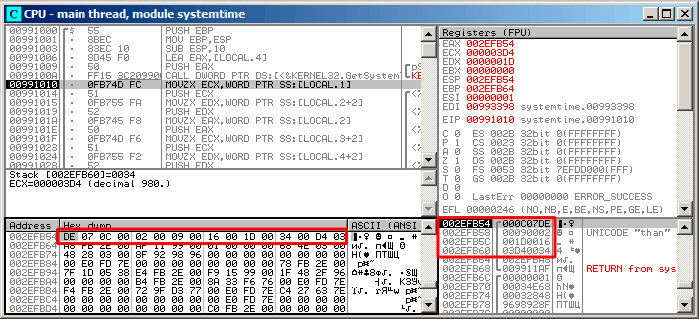
\includegraphics[scale=\FigScale]{patterns/15_structs/1_systemtime/olly_systemtime1.png}
\caption{\olly: \TT{GetSystemTime()} \RU{только что исполнилась}\EN{just executed}}
\label{fig:struct_olly_1}
\end{figure}

\RU{Точное системное время на моем компьютере, в которое исполнилась функция, это}
\EN{The system time of the function execution on my computer is} 9 \RU{декабря}\EN{december} 2014, 22:29:52:

\begin{figure}[H]
\centering
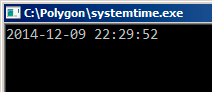
\includegraphics[scale=\NormalScale]{patterns/15_structs/1_systemtime/olly_systemtime2.png}
\caption{\olly: \RU{Вывод \printf}\EN{\printf output}}
\label{fig:struct_olly_2}
\end{figure}

\RU{Таким образом, в окне данных мы видим следующие 16 байт}\EN{So we see these 16 bytes in the
data window}: 
\begin{lstlisting}
DE 07 0C 00 02 00 09 00 16 00 1D 00 34 00 D4 03
\end{lstlisting}

\RU{Каждые два байта отражают одно поле структуры}\EN{Each two bytes represent one field of the structure}. 
\RU{А так как порядок байт (\gls{endianness}) \IT{little endian},
то в начале следует младший байт, затем старший}\EN{Since the \gls{endianness} is \IT{little endian}, 
we see the low byte first and then the high one}.
\RU{Следовательно, вот какие 16-битные числа сейчас записаны в памяти}
\EN{Hence, these are the values currently stored in memory}:

\begin{center}
\begin{tabular}{ | l | l | l | }
\hline
\headercolor{} \RU{Шестнадцатеричное число}\EN{Hexadecimal number} & 
\headercolor{} \RU{десятичное число}\EN{decimal number} & 
\headercolor{} \RU{имя поля}\EN{field name} \\
\hline
0x07DE & 2014	& wYear \\
\hline
0x000C & 12	& wMonth \\
\hline
0x0002 & 2	& wDayOfWeek \\
\hline
0x0009 & 9	& wDay \\
\hline
0x0016 & 22	& wHour \\
\hline
0x001D & 29	& wMinute \\
\hline
0x0034 & 52	& wSecond \\
\hline	
0x03D4 & 980	& wMilliseconds \\
\hline
\end{tabular}
\end{center}

\RU{В окне стека, видны те же значения, только они сгруппированы как 32-битные значения}
\EN{The same values are seen in the stack window, but they are grouped as 32-bit values}.

\RU{Затем}\EN{And then} \printf \RU{просто берет нужные значения и выводит их на консоль}
\EN{just takes the values it needs and outputs them to the console}.

\RU{Некоторые поля}\EN{Some values aren't output by} \printf \RU{не выводит} (\TT{wDayOfWeek} \AndENRU 
\TT{wMilliseconds}), \RU{но они находятся в памяти и доступны для использования.}
\EN{but they are in memory right now, available for use.}

\fi

\subsection{\RU{Замена структуры массивом}\EN{Replacing the structure with array}}

\RU{Тот факт, что поля структуры\EMDASH{}это просто переменные расположенные рядом, легко проиллюстрировать следующим образом.}%
\EN{The fact that the structure fields are just variables located side-by-side, can be easily demonstrated by doing the following.}
\RU{Глядя на описание структуры \TT{SYSTEMTIME}, можно переписать этот простой пример так:}%
\EN{Keeping in mind the \TT{SYSTEMTIME} structure description, it's possible to rewrite this simple example like this:}

\lstinputlisting{patterns/15_structs/1_systemtime/systemtime2.c}

\RU{Компилятор немного ворчит:}\EN{The compiler grumbles a bit:}

\begin{lstlisting}
systemtime2.c(7) : warning C4133: 'function' : incompatible types - from 'WORD [8]' to 'LPSYSTEMTIME'
\end{lstlisting}

\RU{Тем не менее, выдает такой код}\EN{But nevertheless, it produces this code}:

\lstinputlisting[caption=\NonOptimizing MSVC 2010]{patterns/15_structs/1_systemtime/systemtime2.asm}

\RU{И это работает так же}\EN{And it works just as the same}!

\RU{Любопытно что результат на ассемблере неотличим от предыдущего}
\EN{It is very interesting that the
result in assembly form cannot be distinguished from the result of the previous compilation}.
\RU{Таким образом, глядя на этот код, 
никогда нельзя сказать с уверенностью, была ли там объявлена структура, либо просто набор переменных.}
\EN{So by looking at this code, one cannot say for sure if there was a structure declared, or an array.} 

\RU{Тем не менее, никто в здравом уме делать так не будет.}
\EN{Nevertheless, no sane person would do it, }
\RU{Потому что это неудобно}\EN{as it is not convenient}. 
\RU{К тому же, иногда, поля в структуре могут меняться разработчиками, переставляться местами, \etc{}.}
\EN{Also the structure fields may be changed by developers, swapped, \etc{}.}

\ifdefined\IncludeOlly
\RU{С \olly этот пример изучать не будем, потому что он будет точно такой же, как и в случае со структурой.}%
\EN{We will not study this example in \olly, because it will be just the same as in the case with the structure.}
\fi

\section{\RU{Выделяем место для структуры через malloc()}\EN{Let's allocate space for a structure using malloc()}}
\label{struct_malloc_example}

\RU{Однако, бывает и так, что проще хранить структуры не в стеке, а в \glslink{heap}{куче}:}
\EN{Sometimes it is simpler to place structures not the in local stack, but in the \gls{heap}:}

\lstinputlisting{patterns/15_structs/2_using_malloc/systemtime_malloc.c}

\RU{Скомпилируем на этот раз с оптимизацией (\Ox) чтобы было проще увидеть то, что нам нужно.}
\EN{Let's compile it now with optimization (\Ox) so it would be easy see what we need.}

\lstinputlisting[caption=\Optimizing MSVC]{patterns/15_structs/2_using_malloc/systemtime_malloc.asm}

\index{\CStandardLibrary!malloc()}
\RU{Итак, \TT{sizeof(SYSTEMTIME) = 16}, именно столько байт выделяется при помощи \TT{malloc()}. 
Она возвращает указатель на только что выделенный блок памяти в \EAX, который копируется в \ESI. 
Win32 функция \TT{GetSystemTime()} обязуется сохранить состояние \ESI, 
поэтому здесь оно нигде не сохраняется и продолжает использоваться после вызова \TT{GetSystemTime()}.}
\EN{So, \TT{sizeof(SYSTEMTIME) = 16} and that is exact number of bytes to be allocated by \TT{malloc()}.
It returns a pointer to a freshly allocated memory block in the \EAX register,
which is then moved into the \ESI register.
\TT{GetSystemTime()} win32 function takes care of saving value in \ESI,
and that is why it is not saved here and continues to be used after the \TT{GetSystemTime()} call.}

\index{x86!\Instructions!MOVZX}
\RU{
Новая инструкция ~--- \MOVZX (\IT{Move with Zero eXtend}). 
Она нужна почти там же где и \MOVSX, 
только всегда очищает остальные биты в 0. Дело в том, что \printf требует 32-битный тип \Tint, 
а в структуре лежит WORD ~--- это 16-битный беззнаковый тип. Поэтому копируя значение из WORD в \Tint, 
нужно очистить биты от 16 до 31, иначе там будет просто случайный мусор, оставшийся от предыдущих действий 
с регистрами.}
\EN{New instruction~---\MOVZX (\IT{Move with Zero eXtend}).
It may be used in most cases as \MOVSX, but it sets the remaining bits to 0.
That's because \printf requires a 32-bit \Tint, but we got a WORD in the structure~---that
is 16-bit unsigned type.
That's why by copying the value from a WORD into \Tint{}, bits from 16 to 31 must be cleared, 
because a random noise may be there, which is left from the previous operations on the register(s).}

\RU{В этом примере можно также представить структуру как массив 8-и WORD-ов:}
\EN{In this example, it's possible to represent the structure as an array of 8 WORDs:}

\lstinputlisting{patterns/15_structs/2_using_malloc/systemtime_malloc2.c}

\RU{Получим такое}\EN{We get}:

\lstinputlisting[caption=\Optimizing MSVC]{patterns/15_structs/2_using_malloc/systemtime_malloc2.asm}

\RU{И снова мы получаем идентичный код, неотличимый от предыдущего.}
\EN{Again, we got the code cannot be distinguished from the previous one.}
\RU{Но и снова нужно отметить, что в реальности так лучше не делать, 
если только вы не знаете точно, что вы делаете.}
\EN{And again it should be noted, you haven't to do this in practice, unless you really know what you are doing.}


\ifx\LITE\undefined
\section{UNIX: struct tm}

% subsections here:
\subsection{Linux}

\RU{В Линуксе, для примера, возьмем структуру \TT{tm} из \TT{time.h}:}
\EN{Let's take the \TT{tm} structure from \TT{time.h} in Linux for example:}

\lstinputlisting{patterns/15_structs/3_tm_linux/GCC_tm.c}

\RU{Компилируем при помощи}\EN{Let's compile it in} GCC 4.4.1:

\lstinputlisting[caption=GCC 4.4.1]{patterns/15_structs/3_tm_linux/GCC_tm.asm.\LANG}

\RU{К сожалению, по какой-то причине, \IDA не сформировала названия локальных переменных в стеке. 
Но так как мы уже опытные реверсеры :-) то можем обойтись и без этого в таком простом примере.}
\EN{Somehow, \IDA did not write the local variables' names in the local stack.
But since we already are experienced reverse engineers :-) we may do it without this information in 
this simple example.}

\index{x86!\Instructions!LEA}
\RU{Обратите внимание на \TT{lea edx, [eax+76Ch]} ~--- эта инструкция прибавляет \TT{0x76C} (1900) к \EAX, 
но не модифицирует флаги. См. также соответствующий раздел об инструкции \LEA{}~(\myref{sec:LEA}).}
\EN{Please also pay attention to the \TT{lea edx, [eax+76Ch]}~---this instruction just adds \TT{0x76C} (1900) to value in \EAX,
but doesn't modify any flags. See also the relevant section about \LEA{}~(\myref{sec:LEA}).}

\ifdefined\IncludeGDB
\subsubsection{GDB}

\RU{Попробуем загрузить пример в GDB}\EN{Let's try to load the example into GDB}
\footnote{\RU{Результат работы \IT{date} немного подправлен в целях демонстрации.}%
\EN{The \IT{date} result is slightly corrected for demonstration purposes.}
\RU{Конечно же, в реальности, нельзя так быстро запустить GDB, чтобы значение секунд осталось бы таким же.}
\EN{Of course, it's not possible to run GDB that quickly, in the same second.}}:

\lstinputlisting[caption=GDB]{patterns/15_structs/3_tm_linux/GCC_tm_GDB.txt}

\RU{Мы легко находим нашу структуру в стеке}\EN{We can easily find our structure in the stack}.
\RU{Для начала, посмотрим, как она объявлена в}\EN{First, let's see how it's defined in} \IT{time.h}:

\begin{lstlisting}[caption=time.h, label=struct_tm]
struct tm
{
  int	tm_sec;
  int	tm_min;
  int	tm_hour;
  int	tm_mday;
  int	tm_mon;
  int	tm_year;
  int	tm_wday;
  int	tm_yday;
  int	tm_isdst;
};
\end{lstlisting}

\RU{Обратите внимание что здесь 32-битные \Tint вместо WORD в SYSTEMTIME}\EN{Pay attention that
32-bit \Tint is used here instead of WORD in SYSTEMTIME}.
\RU{Так что, каждое поле занимает 32-битное слово}\EN{So, each field occupies 32-bit}.

\RU{Вот поля нашей структуры в стеке}\EN{Here are the fields of our structure in the stack}:

\begin{lstlisting}
0xbffff0dc:	0x080484c3	0x080485c0	0x000007de	0x00000000
0xbffff0ec:	0x08048301	0x538c93ed	0x00000025 sec	0x0000000a min
0xbffff0fc:	0x00000012 hour	0x00000002 mday	0x00000005 mon 	0x00000072 year
0xbffff10c:	0x00000001 wday	0x00000098 yday	0x00000001 isdst0x00002a30
0xbffff11c:	0x0804b090	0x08048530	0x00000000	0x00000000
\end{lstlisting}

\RU{Либо же, в виде таблицы}\EN{Or as a table}:

\begin{center}
\begin{tabular}{ | l | l | l | }
\hline
\headercolor{} \RU{Шестнадцатеричное число}\EN{Hexadecimal number} & 
\headercolor{} \RU{десятичное число}\EN{decimal number} & 
\headercolor{} \RU{имя поля}\EN{field name} \\
\hline
0x00000025 & 37 	& tm\_sec \\
\hline
0x0000000a & 10 	& tm\_min \\
\hline
0x00000012 & 18 	& tm\_hour \\	
\hline
0x00000002 & 2 		& tm\_mday \\	
\hline
0x00000005 & 5 		& tm\_mon \\	
\hline
0x00000072 & 114 	& tm\_year \\
\hline
0x00000001 & 1 		& tm\_wday \\	
\hline
0x00000098 & 152 	& tm\_yday \\	
\hline
0x00000001 & 1 		& tm\_isdst \\
\hline
\end{tabular}
\end{center}

\RU{Как и в примере с}\EN{Just like} SYSTEMTIME (\myref{sec:SYSTEMTIME}), 
\RU{здесь есть и другие поля, готовые для использования, 
но в нашем примере они не используются, например,}
\EN{there are also other fields available that are not used, like} tm\_wday, tm\_yday, tm\_isdst.
\fi

\ifdefined\IncludeARM
\subsection{ARM}

\subsubsection{\OptimizingKeilVI (\ThumbMode)}

\RU{Этот же пример}\EN{Same example}:

\lstinputlisting[caption=\OptimizingKeilVI (\ThumbMode)]{patterns/15_structs/3_tm_linux/ARM/tm_ARM_keil_thumb.asm}

\subsubsection{\OptimizingXcodeIV (\ThumbTwoMode)}

\IDA \q{\RU{узнала}\EN{knows}} \RU{структуру}\EN{the} \TT{tm}\EN{ structure} 
(\RU{потому что}\EN{because} \IDA \q{\RU{знает}\EN{knows}} \RU{типы аргументов библиотечных функций, 
таких как}\EN{the types of the arguments of library functions like} \TT{localtime\_r()}), 
\RU{поэтому показала здесь обращения к отдельным элементам структуры и присвоила им имена}
\EN{so it shows here structure elements accesses and their names}.

\lstinputlisting[caption=\OptimizingXcodeIV (\ThumbTwoMode)]{patterns/15_structs/3_tm_linux/ARM/tm_ARM_xcode_thumb.asm}

\fi
\ifdefined\IncludeMIPS
\subsection{MIPS}

\lstinputlisting[caption=\Optimizing GCC 4.4.5 (IDA),numbers=left]{patterns/15_structs/3_tm_linux/MIPS/MIPS_O3_IDA.lst.\LANG}

\RU{Это тот пример, где branch delay slot-ы могут нас запутать.}
\EN{This is an example where the branch delay slots can confuse us.}
\RU{Например, в строке 35 есть инструкция \q{addiu \$a1, 1900}, добавляющая 1900 к числу года.}
\EN{For example, there is the instruction \q{addiu \$a1, 1900} at line 35 which adds 1900 to the year number.}
\RU{Но она исполняется перед исполнением соответствующей JALR в строке 34, не забыайте.}
\EN{It's executed before the corresponding JALR at line 34, do not forget about it.}

\fi
% subsection:
\ifdefined\IncludeGCC
\subsection{\RU{Структура как набор переменных}\EN{Structure as a set of values}}

\RU{Чтобы проиллюстрировать то что структура ~--- это просто набор переменных, лежащих в одном месте, 
переделаем немного пример, еще раз заглянув в описание структуры \IT{tm}}
\EN{In order to illustrate that the structure is just variables laying side-by-side in one place, 
let's rework our example while looking at the \IT{tm} structure definition again}: \lstref{struct_tm}.

\lstinputlisting{patterns/15_structs/3_tm_linux/as_array/GCC_tm2.c}

\index{\CStandardLibrary!localtime\_r()}
N.B. \RU{В \TT{localtime\_r} передается указатель именно на \TT{tm\_sec}, 
т.е. на первый элемент \q{структуры}.}
\EN{The pointer to the \TT{tm\_sec} field is passed into \TT{localtime\_r}, i.e., 
to the first element of the \q{structure}.}

\RU{В итоге, и этот компилятор поворчит}\EN{The compiler warns us}:

\begin{lstlisting}[caption=GCC 4.7.3]
GCC_tm2.c: In function 'main':
GCC_tm2.c:11:5: warning: passing argument 2 of 'localtime_r' from incompatible pointer type [enabled by default]
In file included from GCC_tm2.c:2:0:
/usr/include/time.h:59:12: note: expected 'struct tm *' but argument is of type 'int *'
\end{lstlisting}

\RU{Тем не менее, сгенерирует такое}\EN{But nevertheless, it generates this}:

\lstinputlisting[caption=GCC 4.7.3]{patterns/15_structs/3_tm_linux/as_array/GCC_tm2.asm}

\RU{Этот код почти идентичен уже рассмотренному, и нельзя сказать, была ли структура
в оригинальном исходном коде либо набор переменных.}\EN{This code is identical to what we saw previously and it is
not possible to say, was it a structure in original source code or just a pack of variables.}

\RU{И это работает}\EN{And this works}. 
\RU{Однако, в реальности так лучше не делать}\EN{However, it is not recommended to do this in practice}. 
\RU{Обычно, неоптимизируюий компилятор располагает переменные в локальном
стеке в том же порядке, в котором они объявляются в функции.}
\EN{Usually, non-optimizing compilers allocates variables in the local stack in the 
same order as they were declared in the function.}
\RU{Тем не менее, никакой гарантии нет.}
\EN{Nevertheless, there is no guarantee.}

\RU{Кстати, какой-нибудь другой компилятор может предупредить, что переменные}
\EN{By the way, some other compiler may warn about the} \TT{tm\_year}, \TT{tm\_mon}, \TT{tm\_mday},
\TT{tm\_hour}, \TT{tm\_min}\RU{, но не}\EN{ variables, but not} \TT{tm\_sec}\RU{, используются без инициализации}
\EN{ are used without being initialized}.
\RU{Действительно, ведь компилятор не знает что они будут заполнены при вызове функции}
\EN{Indeed, the compiler is not aware that these are to be filled by} 
\TT{localtime\_r()}\EN{ function}.

\EN{We chose this example, since all structure fields are of type \Tint.}%
\RU{Мы выбрали именно этот пример для иллюстрации, потому что все члены структуры имеют тип \Tint.}
\RU{Это не сработает, если поля структуры будут иметь размер 16 бит (\TT{WORD}), как в случае
со структурой \TT{SYSTEMTIME}}\EN{This would not work if structure fields are 16-bit (\TT{WORD}), 
like in the case of the \TT{SYSTEMTIME} structure}\EMDASH{}\TT{GetSystemTime()} 
\RU{заполнит их неверно}\EN{will fill them incorrectly} 
(\RU{потому что локальные переменные выровнены по 32-битной границе}
\EN{because the local variables are aligned on a 32-bit boundary}).
\RU{Читайте об этом в следующей секции}\EN{Read more about it in next section}: 
\q{\StructurePackingSectionName} (\myref{structure_packing}).

\RU{Так что, структура\EMDASH{}это просто набор переменных лежащих в одном месте, рядом.}%
\EN{So, a structure is just a pack of variables laying on one place, side-by-side.}
\RU{Можно было бы сказать, что структура\EMDASH{}это инструкция компилятору, заставляющая его удерживать переменные в одном месте.}%
\EN{We could say that the structure is the instruction to the compiler, directing it to hold variables in one place.}
\RU{Кстати, когда-то, в очень ранних версиях Си (перед 1972) структур не было вовсе}%
\EN{By the way, in some very early C versions (before 1972), there were no structures at all} \cite{Ritchie:1993:DCL:155360.155580}.

\RU{Здесь нет примера с отладчиком: потому что он будет полностью идентичным тому, что вы уже видели.}%
\EN{There is no debugger example here: it is just the same as you already saw.}

\subsection{\RU{Структура как массив 32-битных слов}\EN{Structure as an array of 32-bit words}}

\lstinputlisting{patterns/15_structs/3_tm_linux/as_array/GCC_tm3.c}

\RU{Мы просто приводим (\IT{cast}) указатель на структуру к массиву \Tint{}-ов}%
\EN{We just \IT{cast} a pointer to structure to an array of \Tint{}'s}.
\RU{И это работает}\EN{And that works}!
\RU{Запускаем пример}\EN{We run the example at} 23:51:45 26-July-2014.

\begin{lstlisting}[label=GCC_tm3_output]
0x0000002D (45)
0x00000033 (51)
0x00000017 (23)
0x0000001A (26)
0x00000006 (6)
0x00000072 (114)
0x00000006 (6)
0x000000CE (206)
0x00000001 (1)
\end{lstlisting}

\RU{Переменные здесь в том же порядке, в котором они перечислены в определении структуры}\EN{The variables here 
are in the same order as they are enumerated in the definition of the structure}: \myref{struct_tm}.

\RU{Вот как это компилируется}\EN{Here is how it gets compiled}:

\lstinputlisting[caption=\Optimizing GCC 4.8.1]{patterns/15_structs/3_tm_linux/as_array/GCC_tm3.lst.\LANG}

\RU{И действительно: место в локальном стеке в начале используется как структура, затем как массив.}
\EN{Indeed: the space in the local stack is first treated as a structure, and then it's treated as an array.}

\RU{Возможно даже модифицировать поля структуры через указатель.}
\EN{It's even possible to modify the fields of the structure through this pointer.}

\RU{И снова, это сомнительный хакерский способ, который не рекомендуется использовать в настоящем коде.}
\EN{And again, it's dubiously hackish way to do things, not recommended for use in production code.}

\ifdefined\IncludeExercises
\myparagraph{\Exercise}

\RU{В качестве упражнения, попробуйте модифицировать (увеличить на 1) 
текущий номер месяца обращаясь со структурой как с массивом.}
\EN{As an exercise, try to modify (increase by 1) the current month number, treating the structure as 
an array.}
\fi

\subsection{\RU{Структура как массив байт}\EN{Structure as an array of bytes}}

\RU{Можно пойти еще дальше. Можно привести (\IT{cast}) указатель к массиву байт и вывести его:}%
\EN{We can go even further. Let's \IT{cast} the pointer to an array of bytes and dump it:}

\lstinputlisting{patterns/15_structs/3_tm_linux/as_array/GCC_tm4.c}

\begin{lstlisting}
0x2D 0x00 0x00 0x00 
0x33 0x00 0x00 0x00 
0x17 0x00 0x00 0x00 
0x1A 0x00 0x00 0x00 
0x06 0x00 0x00 0x00 
0x72 0x00 0x00 0x00 
0x06 0x00 0x00 0x00 
0xCE 0x00 0x00 0x00 
0x01 0x00 0x00 0x00 
\end{lstlisting}

\RU{Мы также запускаем этот пример в}\EN{We also run this example also at} 23:51:45 26-July-2014
\footnote{\EN{The time and date are the same for demonstration purposes. Byte values are fixed up.}%
\RU{Время и дата такая же в целях демонстрации. Значения байт были подправлены.}}.
\RU{Переменные точно такие же, как и в предыдущем выводе}\EN{The values are just the same as in the previous dump} 
(\myref{GCC_tm3_output}), \RU{и конечно, младший байт идет в самом начале, потому что это архитектура 
little-endian}\EN{and of course, the lowest byte goes first, because this is a little-endian architecture} 
(\myref{sec:endianness}).

\lstinputlisting[caption=\Optimizing GCC 4.8.1]{patterns/15_structs/3_tm_linux/as_array/GCC_tm4.lst.\LANG}
\fi


\fi
\section{\StructurePackingSectionName}
\label{structure_packing}

\RU{Достаточно немаловажный момент, это упаковка полей в структурах\footnote{См. также: \URLWPDA}.}
\EN{One important thing is fields packing in structures\footnote{See also: \URLWPDA}.}

\RU{Возьмем простой пример:}\EN{Let's take a simple example:}

\lstinputlisting{patterns/15_structs/4_packing/packing.c}

\RU{Как видно, мы имеем два поля \Tchar (занимающий один байт) и еще два ~--- \Tint (по 4 байта).}
\EN{As we see, we have two \Tchar fields (each is exactly one byte) and two more~---\Tint (each --- 4 bytes).}

% subsections:

\subsection{x86}

\RU{Компилируется это все в:}\EN{This compiles to:}

\lstinputlisting[caption=MSVC 2012 /GS- /Ob0,label=src:struct_packing_4,numbers=left]{patterns/15_structs/4_packing/packing.asm.\LANG}

\RU{Кстати, мы передаем всю структуру, но в реальности, как видно, структура в начале копируется
во временную структуру (выделение места под нее в стеке происходит в строке 10,
а все 4 поля, по одному, копируются в строках 12 \ldots\ 19), 
затем передается только указатель на нее (или адрес).}
\EN{We pass the structure as a whole, but in fact, as we can see, the structure
is being copied to a temporary one (a place in stack is allocated in line 10 for it,
and then all 4 fields, one by one, are copied in lines 12 \ldots\ 19), 
and then its pointer (address) is to be passed.}
\RU{Структура копируется, потому что неизвестно, будет ли функция \ttf модифицировать структуру или нет.
И если да, то структура внутри \main должна остаться той же.}
\EN{The structure is copied because it's not known whether the \ttf{} 
function going to modify the structure or not.
If it gets changed, then the structure in \main has to remain as it was.}
\RU{Мы могли бы использовать указатели на \CCpp, и итоговый код был бы почти такой же,
только копирования не было бы.}
\EN{We could use \CCpp pointers, and the resulting code will be almost the same, but without
the copying.}

\RU{Мы видим здесь что адрес каждого поля в структуре выравнивается по 4-байтной границе. 
Так что каждый \Tchar здесь занимает те же 4 байта что и \Tint. Зачем? 
Затем что процессору удобнее обращаться по таким адресам и кэшировать данные из памяти.}
\EN{As we can see, each field's address is aligned on a 4-byte boundary.
That's why each \Tchar occupies 4 bytes here (like \Tint). Why?
Because it is easier for the CPU to access memory at aligned addresses and to cache data from it.}

\RU{Но это не экономично по размеру данных.}\EN{However, it is not very economical.}

\RU{Попробуем скомпилировать тот же исходник с опцией}\EN{Let's try to compile it with option} (\TT{/Zp1}) 
(\IT{/Zp[n] pack structures on n-byte boundary}).

\lstinputlisting[caption=MSVC 2012 /GS- /Zp1,label=src:struct_packing_1,numbers=left]
{patterns/15_structs/4_packing/packing_msvc_Zp1.asm.\LANG}

\RU{Теперь структура занимает 10 байт и все \Tchar занимают по байту. Что это дает? 
Экономию места. Недостаток ~--- процессор будет обращаться к этим полям не так эффективно 
по скорости, как мог бы.}
\EN{Now the structure takes only 10 bytes and each \Tchar value takes 1 byte. What does it give to us?
Size economy. And as drawback~---the CPU accessing these fields slower than it could.}

\label{short_struct_copying_using_MOV}
\RU{Структура так же копируется в \main. Но не по одному полю, а 10 байт, при помощи трех
пар \MOV.}
\EN{The structure is also copied in \main. Not field-by-field, but directly 10 bytes, using three pairs
of \MOV.}
\RU{Почему не 4?}\EN{Why not 4?}
\RU{Компилятор рассудил, что будет лучше скопировать 10 байт
при помощи 3 пар \MOV, чем копировать два 32-битных слова и два байта при помощи 4 пар \MOV.}
\EN{The compiler decided that it's better to copy 10 bytes using 3 \MOV pairs than to copy two 32-bit words
and two bytes using 4 \MOV pairs.}
\ifx\LITE\undefined
\RU{Кстати, подобная реализация копирования при помощи \MOV взамен вызова функции \TT{memcpy()}, например, это
очень распространенная практика, потому что это в любом случае работает быстрее чем вызов \TT{memcpy()} ---
если речь идет о коротких блоках, конечно: \myref{copying_short_blocks}.}
\EN{By the way, such copy implementation using \MOV instead of calling the \TT{memcpy()} function is widely
used, because it's faster than a call to \TT{memcpy()}---for short blocks, of course:
\myref{copying_short_blocks}.}
\fi

\RU{Как нетрудно догадаться, если структура используется много в каких исходниках и объектных файлах, 
все они должны быть откомпилированы с одним и тем же соглашением об упаковке структур.}
\EN{As it can be easily guessed, if the structure is used in many source and object files,
all these must be compiled with the same convention about structures packing.}

\newcommand{\FNURLMSDNZP}{\footnote{\href{http://go.yurichev.com/17067}
{MSDN: Working with Packing Structures}}}
\newcommand{\FNURLGCCPC}{\footnote{\href{http://go.yurichev.com/17068}
{Structure-Packing Pragmas}}}

\RU{Помимо ключа MSVC \TT{/Zp}, указывающего, по какой границе упаковывать поля структур, есть также 
опция компилятора \TT{\#pragma pack}, её можно указывать прямо в исходнике. 
Это справедливо и для MSVC\FNURLMSDNZP и GCC\FNURLGCCPC{}.}
\EN{Aside from MSVC \TT{/Zp} option which sets how to align each structure field, there is also
the \TT{\#pragma pack} compiler option, which can be defined right in the source code.
It is available in both MSVC\FNURLMSDNZP and GCC\FNURLGCCPC{}.}

\RU{Давайте теперь вернемся к \TT{SYSTEMTIME}, которая состоит из 16-битных полей. 
Откуда наш компилятор знает что их надо паковать по однобайтной границе?}
\EN{Let's get back to the \TT{SYSTEMTIME} structure that consists of 16-bit fields.
How does our compiler know to pack them on 1-byte alignment boundary?}

\RU{В файле \TT{WinNT.h} попадается такое:}\EN{\TT{WinNT.h} file has this:}

\begin{lstlisting}[caption=WinNT.h]
#include "pshpack1.h"
\end{lstlisting}

\RU{И такое:}\EN{And this:}

\begin{lstlisting}[caption=WinNT.h]
#include "pshpack4.h"                   // 4 byte packing is the default
\end{lstlisting}

\RU{Сам файл PshPack1.h выглядит так:}\EN{The file PshPack1.h looks like:}

\begin{lstlisting}[caption=PshPack1.h]
#if ! (defined(lint) || defined(RC_INVOKED))
#if ( _MSC_VER >= 800 && !defined(_M_I86)) || defined(_PUSHPOP_SUPPORTED)
#pragma warning(disable:4103)
#if !(defined( MIDL_PASS )) || defined( __midl )
#pragma pack(push,1)
#else
#pragma pack(1)
#endif
#else
#pragma pack(1)
#endif
#endif /* ! (defined(lint) || defined(RC_INVOKED)) */
\end{lstlisting}

\RU{Собственно, так и задается компилятору, как паковать объявленные после \TT{\#pragma pack} структуры.}
\EN{This tell the compiler how to pack the structures defined after \TT{\#pragma pack}.}

\ifdefined\IncludeOlly
\clearpage
\subsubsection{\olly + \RU{упаковка полей по умолчанию}\EN{fields are packed by default}}
\index{\olly}

\RU{Попробуем в \olly наш пример, где поля выровнены по умолчанию (4 байта)}
\EN{Let's try our example (where the fields are aligned by default (4 bytes)) in \olly}:

\begin{figure}[H]
\centering
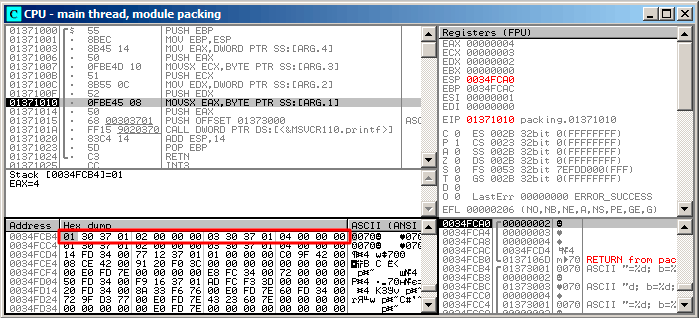
\includegraphics[scale=\FigScale]{patterns/15_structs/4_packing/olly_packing_4.png}
\caption{\olly: \RU{Перед исполнением \printf}\EN{Before \printf execution}}
\label{fig:packing_olly_4}
\end{figure}

\RU{В окне данных видим наши четыре поля}\EN{We see our 4 fields in the data window}.
\RU{Вот только, откуда взялись случайные байты (0x30, 0x37, 0x01) рядом с первым (a) и третьим (c) полем?}
\EN{But where do the random bytes (0x30, 0x37, 0x01) come from, that are next to the first (a) and third (c) fields?}
\RU{Если вернетесь к листингу \myref{src:struct_packing_4}, то увидите, что первое и третье поле имеет
тип \Tchar, а следовательно, туда записывается только один байт, 1 и 3 соответственно (строки 6 и 8).}
\EN{By looking at our listing \myref{src:struct_packing_4}, we can see that the first and third fields
are \Tchar, therefore only one byte is written, 1 and 3 respectively (lines 6 and 8).}
\RU{Остальные три байта 32-битного слова не будут модифицироваться в памяти!}
\EN{The remaining 3 bytes of the 32-bit words are not being modified in memory!}
\RU{А, следовательно, там остается случайный мусор.}\EN{Hence, random garbage is left there.}
\index{x86!\Instructions!MOVSX}
\RU{Этот мусор никак не будет влиять на работу \printf,
потому что значения для нее готовятся при помощи инструкции \MOVSX, которая загружает
из памяти байты а не слова}
\EN{This garbage doesn't influence the \printf output in any way, because the values for it are prepared
using the \MOVSX instruction, which takes bytes, not words}: 
\lstref{src:struct_packing_4} (\RU{строки}\EN{lines} 34 \AndENRU 38).

\RU{Кстати, здесь используется именно \MOVSX (расширяющая знак), потому что тип 
\Tchar\EMDASH{}знаковый по умолчанию в MSVC и GCC.}
\EN{By the way, the \MOVSX (sign-extending) instruction is used here, because 
\Tchar is signed by default in MSVC and GCC.}
\RU{Если бы здесь был тип}\EN{If the type} \TT{unsigned char} \OrENRU \TT{uint8\_t}\EN{ was used here}, 
\RU{то здесь была бы инструкция \MOVZX}\EN{\MOVZX instruction would have been used instead}.

\clearpage
\subsubsection{\olly + \RU{упаковка полей по границе в 1 байт}\EN{fields aligning on 1 byte boundary}}
\index{\olly}

\RU{Здесь всё куда понятнее: 4 поля занимают 10 байт и значения сложены в памяти друг к другу}
\EN{Things are much clearer here: 4 fields occupy 10 bytes and the values are stored side-by-side}

\begin{figure}[H]
\centering
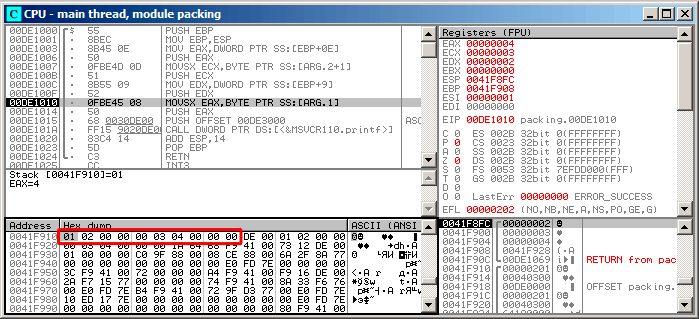
\includegraphics[scale=\FigScale]{patterns/15_structs/4_packing/olly_packing_1.png}
\caption{\olly: \RU{Перед исполнением \printf}\EN{Before \printf execution}}
\label{fig:packing_olly_1}
\end{figure}

\fi


\ifdefined\IncludeARM
\subsection{ARM}

\subsubsection{\OptimizingKeilVI (\ThumbMode)}

\lstinputlisting[caption=\OptimizingKeilVI (\ThumbMode)]{patterns/15_structs/4_packing/packing_Keil_thumb.asm}

\RU{Как мы помним, здесь передается не указатель на структуру, а сама структура, а так как в ARM первые 4 аргумента
функции передаются через регистры, то поля структуры передаются через}
\EN{As we may recall, here a structure is passed instead of pointer to one,
and since the first 4 function arguments in ARM are passed via registers,
the structure's fields are passed via} \TT{R0-R3}.

\index{ARM!\Instructions!LDRB}
\index{x86!\Instructions!MOVSX}
\RU{Инструкция }\TT{LDRB} \RU{загружает один байт из памяти и расширяет до 32-бит учитывая знак.}
\EN{loads one byte from memory and extends it to 32-bit, taking its sign into account.}
\RU{Это то же что и инструкция}\EN{This is similar to} \MOVSX \RU{в}\EN{in} x86.
\RU{Она здесь применяется для загрузки полей}\EN{Here it is used to load fields} $a$ \AndENRU $c$ 
\RU{из структуры}\EN{from the structure}.

\index{Function epilogue}
\RU{Еще что бросается в глаза, так это то что вместо эпилога функции, переход на эпилог другой функции!}
\EN{One more thing we spot easily is that instead of function epilogue, there is jump to another function's epilogue!}
\RU{Действительно, то была совсем другая, не относящаяся к этой, функция, однако, она имела точно такой же
эпилог}\EN{Indeed, that was quite different function, not related in any way to ours, however, it has exactly
the same epilogue} 
(\RU{видимо, тоже хранила в стеке 5 локальных переменных}\EN{probably because, it hold 5 local variables too} 
($5*4=0x14$)).
\RU{К тому же, она находится рядом (обратите внимание на адреса).}
\EN{Also it is located nearby (take a look at the addresses).}
\RU{Действительно, нет никакой разницы, какой эпилог исполнять, если он работает так же, как нам нужно.}
\EN{Indeed, it doesn't matter which epilogue gets executed,
if it works just as we need.}
\RU{Keil решил использовать часть другой функции, вероятно, из-за экономии.}
\EN{Apparently, Keil decides to reuse a part of another function to economize.}
\RU{Эпилог занимает 4 байта, а переход ~--- только 2.}
\EN{The epilogue takes 4 bytes while jump~---only 2.}

\subsubsection{ARM + \OptimizingXcodeIV (\ThumbTwoMode)}

\lstinputlisting[caption=\OptimizingXcodeIV (\ThumbTwoMode)]{patterns/15_structs/4_packing/packing_Xcode_thumb.asm}

\index{ARM!\Instructions!SXTB}
\index{x86!\Instructions!MOVSX}
\TT{SXTB} (\IT{Signed Extend Byte}) \RU{это также аналог}\EN{is analogous to} \MOVSX \InENRU x86.
\RU{Всё остальное ~--- так же.}\EN{All the rest~---just the same.}

\fi
\ifdefined\IncludeMIPS
\subsection{MIPS}
\label{MIPS_structure_big_endian}

\lstinputlisting[caption=\Optimizing GCC 4.4.5 (IDA),numbers=left]{patterns/15_structs/4_packing/MIPS_O3_IDA.lst}

\RU{Поля структуры приходят в регистрах \$A0..\$A3 и затем перетасовываются в регистры \$A1..\$A4 для \printf.}
\EN{Structure fields come in registers \$A0..\$A3 and then get reshuffled into \$A1..\$A4 for \printf.}
\RU{Но здесь есть две инструкции SRA (\q{Shift Word Right Arithmetic}), которые готовят поля типа \Tchar.}
\EN{But there are two SRA (\q{Shift Word Right Arithmetic}) instructions, which prepare \Tchar fields.}
\RU{Почему}\EN{Why}?
\RU{По умолчанию, MIPS это big-endian архитектура \myref{sec:endianness}, и Debian Linux в котором мы работаем, также big-endian.}
\EN{MIPS is a big-endian architecture by default \myref{sec:endianness}, and the Debian Linux we work in is big-endian as well.}
\RU{Так что когда один байт расположен в 32-битном элементе структуры, он занимает биты 31..24.}
\EN{So when byte variables are stored in 32-bit structure slots, they occupy the high 31..24 bits.}
\RU{И когда переменную типа \Tchar нужно расширить до 32-битного значения, она должна быть сдвинута вправо
на 24 бита.}
\EN{And when a \Tchar variable needs to be extended into a 32-bit value, it must be shifted right by 24 bits.}
\RU{\Tchar это знаковый тип, так что здесь нужно использовать арифметический сдвиг вместо логического.}
\EN{\Tchar is a signed type, so an arithmetical shift is used here instead of logical.}

\fi

\subsection{\RU{Еще кое-что}\EN{One more word}}

\EN{Passing a structure as a function argument (instead of a passing pointer to structure) is the same
as passing all structure fields one by one.}
\RU{Передача структуры как аргумент функции (вместо передачи указателя на структуру) это то же
что и передача всех полей структуры по одному.}
\EN{If the structure fields are packed by default, the f() function can be rewritten as:}
\RU{Если поля в структуре пакуются по умолчанию, то функцию f() можно переписать так:}

\begin{lstlisting}
void f(char a, int b, char c, int d)
{
    printf ("a=%d; b=%d; c=%d; d=%d\n", a, b, c, d);
};
\end{lstlisting}

\RU{И в итоге будет такой же код}\EN{And that leads to the same code}.

\section{\RU{Вложенные структуры}\EN{Nested structures}}

\RU{Теперь, как насчет ситуаций, когда одна структура определена внутри другой структуры?}
\EN{Now what about situations when one structure is defined inside of another?}

\lstinputlisting{patterns/15_structs/5_nested/nested.c}

\dots \RU{в этом случае, оба поля \TT{inner\_struct} просто будут располагаться между полями a,b и d,e в 
\TT{outer\_struct}.}
\EN{in this case, both \TT{inner\_struct} fields are to be placed between the a,b and d,e fields of
the \TT{outer\_struct}.}

\RU{Компилируем}\EN{Let's compile} (MSVC 2010):

\lstinputlisting[caption=\Optimizing MSVC 2010 /Ob0]{patterns/15_structs/5_nested/nested_msvc.asm}

\RU{Очень любопытный момент в том, что глядя на этот код на ассемблере, мы даже не видим, 
что была использована какая-то еще другая структура внутри этой!
Так что, пожалуй, можно сказать, что все вложенные структуры в итоге разворачиваются в одну, \IT{линейную} 
или \IT{одномерную} структуру.}
\EN{One curious thing here is that by looking onto this assembly code, we do not even see that
another structure was used inside of it!
Thus, we would say, nested structures are unfolded into \IT{linear} or \IT{one-dimensional} structure.}

\RU{Конечно, если заменить объявление \TT{struct inner\_struct c;} на \TT{struct inner\_struct *c;} 
(объявляя таким образом указатель), ситуация будет совсем иная.}
\EN{Of course, if we replace the \TT{struct inner\_struct c;} declaration with \TT{struct inner\_struct *c;} 
(thus making a pointer here) the situation will be quite different.}
% FIXME1: нарисовать вложенную структуру и развернутую

\ifdefined\IncludeOlly
\clearpage
\subsection{\olly}
\index{\olly}

\RU{Загружаем пример в}\EN{Let's load the example into} \olly \RU{и смотрим на}\EN{and take a look at} 
\TT{outer\_struct} \RU{в памяти}\EN{in memory}:

\begin{figure}[H]
\centering
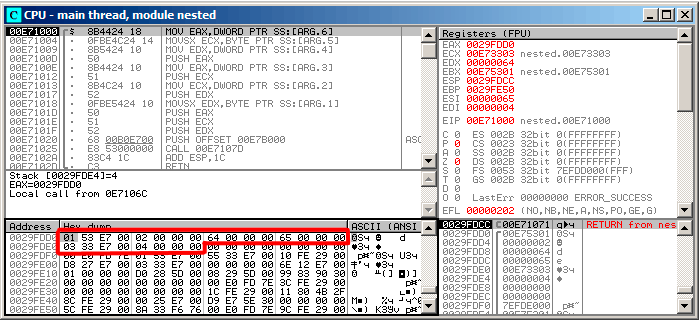
\includegraphics[scale=\FigScale]{patterns/15_structs/5_nested/olly.png}
\caption{\olly: \RU{Перед исполнением \printf}\EN{Before \printf execution}}
\label{fig:nested_olly}
\end{figure}

\RU{Вот как расположены значения в памяти}\EN{That's how the values are located in memory}:
\begin{itemize}
\item \IT{(outer\_struct.a)} \RU{(байт) 1 + 3 байта случайного мусора}\EN{(byte) 1 + 3 bytes of random garbage};
\item \IT{(outer\_struct.b)} (\RU{32-битное слово}\EN{32-bit word}) 2;
\item \IT{(inner\_struct.a)} (\RU{32-битное слово}\EN{32-bit word}) 0x64 (100);
\item \IT{(inner\_struct.b)} (\RU{32-битное слово}\EN{32-bit word}) 0x65 (101);
\item \IT{(outer\_struct.d)} \RU{(байт) 3 + 3 байта случайного мусора}\EN{(byte) 3 + 3 bytes of random garbage};
\item \IT{(outer\_struct.e)} (\RU{32-битное слово}\EN{32-bit word}) 4.
\end{itemize}

\fi


\section{\RU{Работа с битовыми полями в структуре}\EN{Bit fields in a structure}}

\subsection{\RU{Пример CPUID}\EN{CPUID example}}

\RU{Язык \CCpp позволяет указывать, сколько именно бит отвести для каждого поля структуры. 
Это удобно если нужно экономить место в памяти. К примеру, для переменной типа \Tbool достаточно одного бита.
Но, это не очень удобно, если нужна скорость.}
\EN{The \CCpp language allows to define the exact number of bits for each structure field.
It is very useful if one needs to save memory space. 
For example, one bit is enough for a \Tbool variable.
But of course, it is not rational if speed is important.}
% FIXME!
% another use of this is to parse binary protocols/packets, for example
% the definition of struct iphdr in include/linux/ip.h

\newcommand{\FNCPUID}{\footnote{\href{http://go.yurichev.com/17069}{wikipedia}}}

\index{x86!\Instructions!CPUID}
\label{cpuid}
\RU{Рассмотрим пример с инструкцией \CPUID\FNCPUID. 
Эта инструкция возвращает информацию о том, какой процессор имеется в наличии и какие возможности он имеет.}
\EN{Let's consider the \CPUID\FNCPUID instruction example.
This instruction returns information about the current CPU and its features.}

\RU{Если перед исполнением инструкции в \EAX будет 1, 
то \CPUID вернет упакованную в \EAX такую информацию о процессоре:}
\EN{If the \EAX is set to 1 before the instruction's execution, 
\CPUID returning this information packed into the \EAX register:}

\begin{center}
\begin{tabular}{ | l | l | }
\hline
3:0 (4 \bitsENRU)& Stepping \\
7:4 (4 \bitsENRU) & Model \\
11:8 (4 \bitsENRU) & Family \\
13:12 (2 \bitsENRU) & Processor Type \\
19:16 (4 \bitsENRU) & Extended Model \\
27:20 (8 \bitsENRU) & Extended Family \\
\hline
\end{tabular}
\end{center}

\newcommand{\FNGCCAS}{\footnote{\href{http://go.yurichev.com/17070}
{\RU{Подробнее о встроенном ассемблере GCC}\EN{More about internal GCC assembler}}}}

\RU{MSVC 2010 имеет макрос для \CPUID, а GCC 4.4.1 ~--- нет. 
Поэтому для GCC сделаем эту функцию сами, используя его встроенный ассемблер\FNGCCAS.}
\EN{MSVC 2010 has \CPUID macro, but GCC 4.4.1 does not.
So let's make this function by ourselves for GCC with the help of its built-in assembler\FNGCCAS.}

\lstinputlisting{patterns/15_structs/6_bitfields/cpuid/CPUID.c}

\RU{После того как \CPUID заполнит \EAX/\EBX/\ECX/\EDX, у нас они отразятся в массиве \TT{b[]}. 
Затем, мы имеем указатель на структуру \TT{CPUID\_1\_EAX}, и мы указываем его на значение 
\EAX из массива \TT{b[]}.}
\EN{After \CPUID fills \EAX/\EBX/\ECX/\EDX, these registers are to be written in the \TT{b[]} array.
Then, we have a pointer to the \TT{CPUID\_1\_EAX} structure and we point it to the value in \EAX from the \TT{b[]} array.}

\RU{Иными словами, мы трактуем 32-битный \Tint как структуру.}
\EN{In other words, we treat a 32-bit \Tint value as a structure.}
\RU{Затем мы читаем отдельные биты из структуры.}\EN{Then we read specific bits from the structure.}

\subsubsection{MSVC}

\RU{Компилируем в MSVC 2008 с опцией \Ox}\EN{Let's compile it in MSVC 2008 with \Ox option}:

\lstinputlisting[caption=\Optimizing MSVC 2008]{patterns/15_structs/6_bitfields/cpuid/CPUID_msvc_Ox.asm}

\index{x86!\Instructions!SHR}
\RU{Инструкция \TT{SHR} сдвигает значение из \EAX на то количество бит, 
которое нужно \IT{пропустить}, то есть, мы игнорируем некоторые биты \IT{справа}.}
\EN{The \TT{SHR} instruction shifting the value in \EAX by the number of bits that must be
\IT{skipped}, e.g., we ignore some bits \IT{at the right side}.}

\index{x86!\Instructions!AND}
\RU{А инструкция \AND очищает биты \IT{слева} которые нам не нужны, или же, говоря иначе, 
она оставляет по маске только те биты в \EAX, которые нам сейчас нужны.}
\EN{The \AND instruction clears the unneeded bits \IT{on the left}, or, in other words, 
leaves only those bits in the \EAX register we need.}

\ifdefined\IncludeOlly
\clearpage
\subsubsection{MSVC + \olly}
\index{\olly}

\RU{Загрузим пример в}\EN{Let's load our example into} \olly 
\RU{и увидим, какие значения были установлены в EAX/EBX/ECX/EDX после
исполнения}\EN{and see, what values are set in EAX/EBX/ECX/EDX after the execution of} CPUID: 

\begin{figure}[H]
\centering
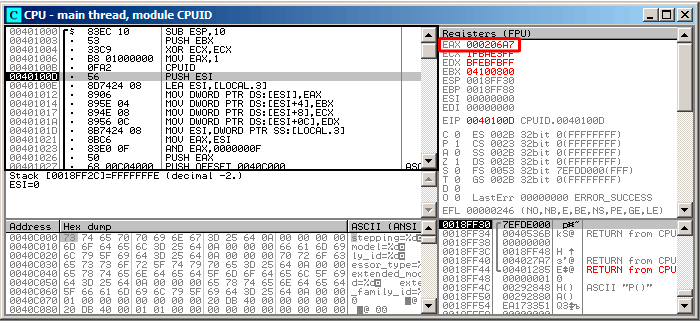
\includegraphics[scale=\FigScale]{patterns/15_structs/6_bitfields/cpuid/olly.png}
\caption{\olly: \RU{После исполнения CPUID}\EN{After CPUID execution}}
\label{fig:cpuid_olly_1}
\end{figure}

\RU{В EAX установлено}\EN{EAX has} \TT{0x000206A7} 
(\RU{мой}\EN{my} \ac{CPU} \EN{is}\RU{---} Intel Xeon E3-1220).\\
\RU{В двоичном виде это}\EN{This is} $0000 0000 0000 0010 0000 0110 1010 0111$\EN{ in binary form}.

\RU{Вот как распределяются биты по полям в моем случае}\EN{Here is how the bits are distributed by fields}:

\begin{center}
\begin{tabular}{ | l | l | l | }
\hline
\headercolor{} \RU{поле}\EN{field} &
\headercolor{} \RU{в двоичном виде}\EN{in binary form} &
\headercolor{} \RU{в десятичном виде}\EN{in decimal form} \\
\hline
reserved2		& 0000 & 0 \\
\hline
extended\_family\_id	& 00000000 & 0 \\
\hline
extended\_model\_id	& 0010 & 2 \\
\hline
reserved1		& 00 & 0 \\
\hline
processor\_id		& 00 & 0 \\
\hline
family\_id		& 0110 & 6 \\
\hline
model			& 1010 & 10 \\
\hline
stepping		& 0111 & 7 \\
\hline
\end{tabular}
\end{center}

\begin{figure}[H]
\centering
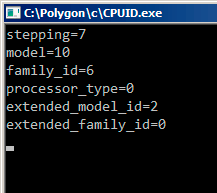
\includegraphics[scale=\NormalScale]{patterns/15_structs/6_bitfields/cpuid/result.png}
\caption{\olly: \RU{Результат работы}\EN{Result}}
\label{fig:cpuid_olly_2}
\end{figure}

\fi

\ifdefined\IncludeGCC
\subsubsection{GCC}

\RU{Попробуем GCC 4.4.1 с опцией \Othree.}\EN{Let's try GCC 4.4.1 with \Othree option.}

\lstinputlisting[caption=\Optimizing GCC 4.4.1]{patterns/15_structs/6_bitfields/cpuid/CPUID_gcc_O3.asm}

\RU{Практически, то же самое. Единственное что стоит отметить это то, что GCC решил зачем-то объединить 
вычисление \TT{extended\_model\_id} и \TT{extended\_family\_id} в один блок, 
вместо того чтобы вычислять их перед соответствующим вызовом \printf.}
\EN{Almost the same.
The only thing worth noting is that GCC somehow combines the calculation of
\TT{extended\_model\_id} and \TT{extended\_family\_id} into one block,
instead of calculating them separately before each \printf call.}
\fi

\ifx\LITE\undefined
\subsection{\WorkingWithFloatAsWithStructSubSubSectionName}
\label{sec:floatasstruct}

\RU{Как уже ранее указывалось в секции о FPU~(\myref{sec:FPU}), 
и \Tfloat и \Tdouble содержат в себе \IT{знак}, \IT{мантиссу} и \IT{экспоненту}. 
Однако, можем ли мы работать с этими полями напрямую? Попробуем с \Tfloat.}
\EN{As we already noted in the section about FPU~(\myref{sec:FPU}), 
both \Tfloat and \Tdouble types consist of a \IT{sign}, 
a \IT{significand} (or \IT{fraction}) and an \IT{exponent}.
But will we be able to work with these fields directly? Let's try this with \Tfloat.}

\bigskip
% a hack used here! http://tex.stackexchange.com/questions/73524/bytefield-package
\begin{center}
\begin{bytefield}{32}
	\bitheader[endianness=big]{0,22,23,30,31} \\
	\bitbox{1}{S} & 
	\bitbox{8}{\RU{экспонента}\EN{exponent}\ESph{}\PTBRph{}\PLph{}} & 
	\bitbox{23}{\RU{мантисса}\EN{mantissa or fraction}\ESph{}\PTBRph{}\PLph{}}
\end{bytefield}
\end{center}

\begin{center}
( S\EMDASH{}\RU{знак}\EN{sign}\ESph{}\PTBRph{}\PLph{} )
\end{center}


\lstinputlisting{patterns/15_structs/6_bitfields/float/float.c.\LANG}

\RU{Структура \TT{float\_as\_struct} занимает в памяти столько же места сколько и \Tfloat, 
то есть 4 байта или 32 бита.}
\EN{The \TT{float\_as\_struct} structure occupies the same amount of  memory as \Tfloat, i.e., 4 bytes or 32 bits.}

\RU{Далее мы выставляем во входящем значении отрицательный знак, 
а также прибавляя двойку к экспоненте, мы тем 
самым умножаем всё значение на \TT{$2^2$}, то есть на 4.}
\EN{Now we are setting the negative sign in the input value and also, by adding 2 to the exponent, 
we thereby multiply the whole number by \TT{$2^2$}, i.e., by 4.}

\RU{Компилируем в MSVC 2008 без включенной оптимизации:}
\EN{Let's compile in MSVC 2008 without optimization turned on:}

\lstinputlisting[caption=\NonOptimizing MSVC 2008]{patterns/15_structs/6_bitfields/float/float_msvc.asm.\LANG}

\RU{Слегка избыточно. В версии скомпилированной с флагом \Ox нет вызовов \TT{memcpy()}, 
там работа происходит сразу с переменной \TT{f}. Но по неоптимизированной версии будет проще понять.}
\EN{A bit redundant.
If it was compiled with \Ox flag there would be no \TT{memcpy()} call,
the \TT{f} variable is used directly.
But it is easier to understand by looking at the unoptimized version.}

\RU{А что сделает GCC 4.4.1 с опцией \Othree?}\EN{What would GCC 4.4.1 with \Othree do?}

\lstinputlisting[caption=\Optimizing GCC 4.4.1]{patterns/15_structs/6_bitfields/float/float_gcc_O3.asm.\LANG}

\RU{Да, функция \ttf в целом понятна. Однако, что интересно, еще при компиляции, 
не взирая на мешанину с полями структуры, GCC умудрился вычислить результат функции \TT{f(1.234)} еще
во время компиляции и сразу подставить его в аргумент для \printf{}!}
\EN{The \ttf function is almost understandable. However, what is interesting is that GCC was able to calculate
the result of \TT{f(1.234)} during compilation despite all this hodge-podge with the structure fields
and prepared this argument to \printf{} as precalculated at compile time!}

\fi

\ifdefined\IncludeExercises
\section{\Exercises}

\subsection{\Exercise \#1}
\label{exercise_struct_1}

\href{http://go.yurichev.com/17217}{Linux x86 (beginners.re)}\footnote{GCC 4.8.1 -O3}\\
\href{http://go.yurichev.com/17218}{Linux MIPS (beginners.re)}\footnote{GCC 4.4.5 -O3}\\
\EN{This program for Linux x86 and Linux MIPS opens a file and prints a number. What is this number?}
\RU{Эта программа для Linux x86 и Linux MIPS открывает файл и выводит какое-то число. Что это за число?}

\Answer{}: \myref{exercise_solutions_struct_1}.

\subsection{\Exercise \#2}
\label{exercise_struct_2}

\EN{This function takes some structure on input and does something. Try to reverse engineer structure field types.
Function contents may be ignored for the moment.}
\RU{Эта функция берет какую-то структуру на вход и делает что-то. Попробуйте разобраться, поля каких типов 
присутствуют в структуре. Самое содержимое функции можно пока игнорировать.}

\begin{lstlisting}[caption=\Optimizing MSVC 2010]
$SG2802	DB	'%f', 0aH, 00H
$SG2803	DB	'%c, %d', 0aH, 00H
$SG2805	DB	'error #2', 0aH, 00H
$SG2807	DB	'error #1', 0aH, 00H

__real@405ec00000000000 DQ 0405ec00000000000r	; 123
__real@407bc00000000000 DQ 0407bc00000000000r	; 444

_s$ = 8
_f	PROC
	push	esi
	mov	esi, DWORD PTR _s$[esp]
	cmp	DWORD PTR [esi], 1000
	jle	SHORT $LN4@f
	cmp	DWORD PTR [esi+4], 10
	jbe	SHORT $LN3@f
	fld	DWORD PTR [esi+8]
	sub	esp, 8
	fmul	QWORD PTR __real@407bc00000000000
	fld	QWORD PTR [esi+16]
	fmul	QWORD PTR __real@405ec00000000000
	faddp	ST(1), ST(0)
	fstp	QWORD PTR [esp]
	push	OFFSET $SG2802 ; '%f'
	call	_printf
	movzx	eax, BYTE PTR [esi+25]
	movsx	ecx, BYTE PTR [esi+24]
	push	eax
	push	ecx
	push	OFFSET $SG2803 ; '%c, %d'
	call	_printf
	add	esp, 24
	pop	esi
	ret	0
$LN3@f:
	pop	esi
	mov	DWORD PTR _s$[esp-4], OFFSET $SG2805 ; 'error #2'
	jmp	_printf
$LN4@f:
	pop	esi
	mov	DWORD PTR _s$[esp-4], OFFSET $SG2807 ; 'error #1'
	jmp	_printf
_f	ENDP
\end{lstlisting}

\begin{lstlisting}[caption=\NonOptimizingKeilVI (\ARMMode)]
f PROC
        PUSH     {r4-r6,lr}
        MOV      r4,r0
        LDR      r0,[r0,#0]
        CMP      r0,#0x3e8
        ADRLE    r0,|L0.140|
        BLE      |L0.132|
        LDR      r0,[r4,#4]
        CMP      r0,#0xa
        ADRLS    r0,|L0.152|
        BLS      |L0.132|
        ADD      r0,r4,#0x10
        LDM      r0,{r0,r1}
        LDR      r3,|L0.164|
        MOV      r2,#0
        BL       __aeabi_dmul
        MOV      r5,r0
        MOV      r6,r1
        LDR      r0,[r4,#8]
        LDR      r1,|L0.168|
        BL       __aeabi_fmul
        BL       __aeabi_f2d
        MOV      r2,r5
        MOV      r3,r6
        BL       __aeabi_dadd
        MOV      r2,r0
        MOV      r3,r1
        ADR      r0,|L0.172|
        BL       __2printf
        LDRB     r2,[r4,#0x19]
        LDRB     r1,[r4,#0x18]
        POP      {r4-r6,lr}
        ADR      r0,|L0.176|
        B        __2printf
|L0.132|
        POP      {r4-r6,lr}
        B        __2printf
        ENDP

|L0.140|
        DCB      "error #1\n",0
        DCB      0
        DCB      0
|L0.152|
        DCB      "error #2\n",0
        DCB      0
        DCB      0
|L0.164|
        DCD      0x405ec000
|L0.168|
        DCD      0x43de0000
|L0.172|
        DCB      "%f\n",0
|L0.176|
        DCB      "%c, %d\n",0
\end{lstlisting}

\begin{lstlisting}[caption=\NonOptimizingKeilVI (\ThumbMode)]
f PROC
        PUSH     {r4-r6,lr}
        MOV      r4,r0
        LDR      r0,[r0,#0]
        CMP      r0,#0x3e8
        ADRLE    r0,|L0.140|
        BLE      |L0.132|
        LDR      r0,[r4,#4]
        CMP      r0,#0xa
        ADRLS    r0,|L0.152|
        BLS      |L0.132|
        ADD      r0,r4,#0x10
        LDM      r0,{r0,r1}
        LDR      r3,|L0.164|
        MOV      r2,#0
        BL       __aeabi_dmul
        MOV      r5,r0
        MOV      r6,r1
        LDR      r0,[r4,#8]
        LDR      r1,|L0.168|
        BL       __aeabi_fmul
        BL       __aeabi_f2d
        MOV      r2,r5
        MOV      r3,r6
        BL       __aeabi_dadd
        MOV      r2,r0
        MOV      r3,r1
        ADR      r0,|L0.172|
        BL       __2printf
        LDRB     r2,[r4,#0x19]
        LDRB     r1,[r4,#0x18]
        POP      {r4-r6,lr}
        ADR      r0,|L0.176|
        B        __2printf
|L0.132|
        POP      {r4-r6,lr}
        B        __2printf
        ENDP

|L0.140|
        DCB      "error #1\n",0
        DCB      0
        DCB      0
|L0.152|
        DCB      "error #2\n",0
        DCB      0
        DCB      0
|L0.164|
        DCD      0x405ec000
|L0.168|
        DCD      0x43de0000
|L0.172|
        DCB      "%f\n",0
|L0.176|
        DCB      "%c, %d\n",0
\end{lstlisting}

\begin{lstlisting}[caption=\Optimizing GCC 4.9 (ARM64)]
f:
	stp	x29, x30, [sp, -32]!
	add	x29, sp, 0
	ldr	w1, [x0]
	str	x19, [sp,16]
	cmp	w1, 1000
	ble	.L2
	ldr	w1, [x0,4]
	cmp	w1, 10
	bls	.L3
	ldr	s1, [x0,8]
	mov	x19, x0
	ldr	s0, .LC1
	adrp	x0, .LC0
	ldr	d2, [x19,16]
	add	x0, x0, :lo12:.LC0
	fmul	s1, s1, s0
	ldr	d0, .LC2
	fmul	d0, d2, d0
	fcvt	d1, s1
	fadd	d0, d1, d0
	bl	printf
	ldrb	w1, [x19,24]
	adrp	x0, .LC3
	ldrb	w2, [x19,25]
	add	x0, x0, :lo12:.LC3
	ldr	x19, [sp,16]
	ldp	x29, x30, [sp], 32
	b	printf
.L3:
	ldr	x19, [sp,16]
	adrp	x0, .LC4
	ldp	x29, x30, [sp], 32
	add	x0, x0, :lo12:.LC4
	b	puts
.L2:
	ldr	x19, [sp,16]
	adrp	x0, .LC5
	ldp	x29, x30, [sp], 32
	add	x0, x0, :lo12:.LC5
	b	puts
	.size	f, .-f
.LC1:
	.word	1138622464
.LC2:
	.word	0
	.word	1079951360
.LC0:
	.string	"%f\n"
.LC3:
	.string	"%c, %d\n"
.LC4:
	.string	"error #2"
.LC5:
	.string	"error #1"
\end{lstlisting}

\lstinputlisting[caption=\Optimizing GCC 4.4.5 (MIPS) (IDA)]{patterns/15_structs/ex2_MIPS_O3_IDA.lst}

\Answer{}: \myref{exercise_solutions_struct_2}.

\fi
